\chapter{Shell Model}
\label{appendix:shell-model}

\section{Shell model}

The idea that an atomic nucleus can have a structure that behaves rather similarly as the atom itself has been enforced by the experimental observations that were done across time. The sharp and discrete discontinuities of nuclear properties, such as the nucleon separation energy, point out that nucleus can be explained through the existence of \emph{shells}. Some examples of observations indicating this are:
\begin{itemize}
    \item When adding a nucleon to a nucleus, there are certain places where the \emph{binding energy} of the next nucleon becomes considerably smaller than the previous one. 
    \item Separation energies for both the protons and neutrons suffer drastic changes, having strong deviations from the predictions of the semi-empirical mass formula \cite{weizsacker1935theorie}, the discontinuities being represented by major shell closures (complete filling) \cite{krane1991introductory}.
    \item The neutron absorption cross-section has a substantial decrease in value at the neutron magic numbers
    \item Great abundance of nuclides where $Z$ and $N$ are magic numbers.
\end{itemize}

The sudden discontinuities occur at specific values of the proton $Z$ and neutron $N$ numbers: these are called \emph{magic numbers}. Currently, these magic numbers correspond to $Z$ or $N=2,8,20,28,50,82,126$, and they represent the major shells. There are also two \emph{weakly magic numbers}: 40 and 64. One can examine the values for the first excited states $2^+$ that are shown in Figs. \ref{e2plus_proton}, \ref{e2plus_neutron}. Indeed, these values show some peaks, each peak corresponding to a particular magic number. This results are part of the work of Raman et al. \cite{raman2001transition}, where the transition probabilities from the ground state to the first-excited $2^+$ state in even-even nuclei were evaluated.
\begin{figure}
    \centering
    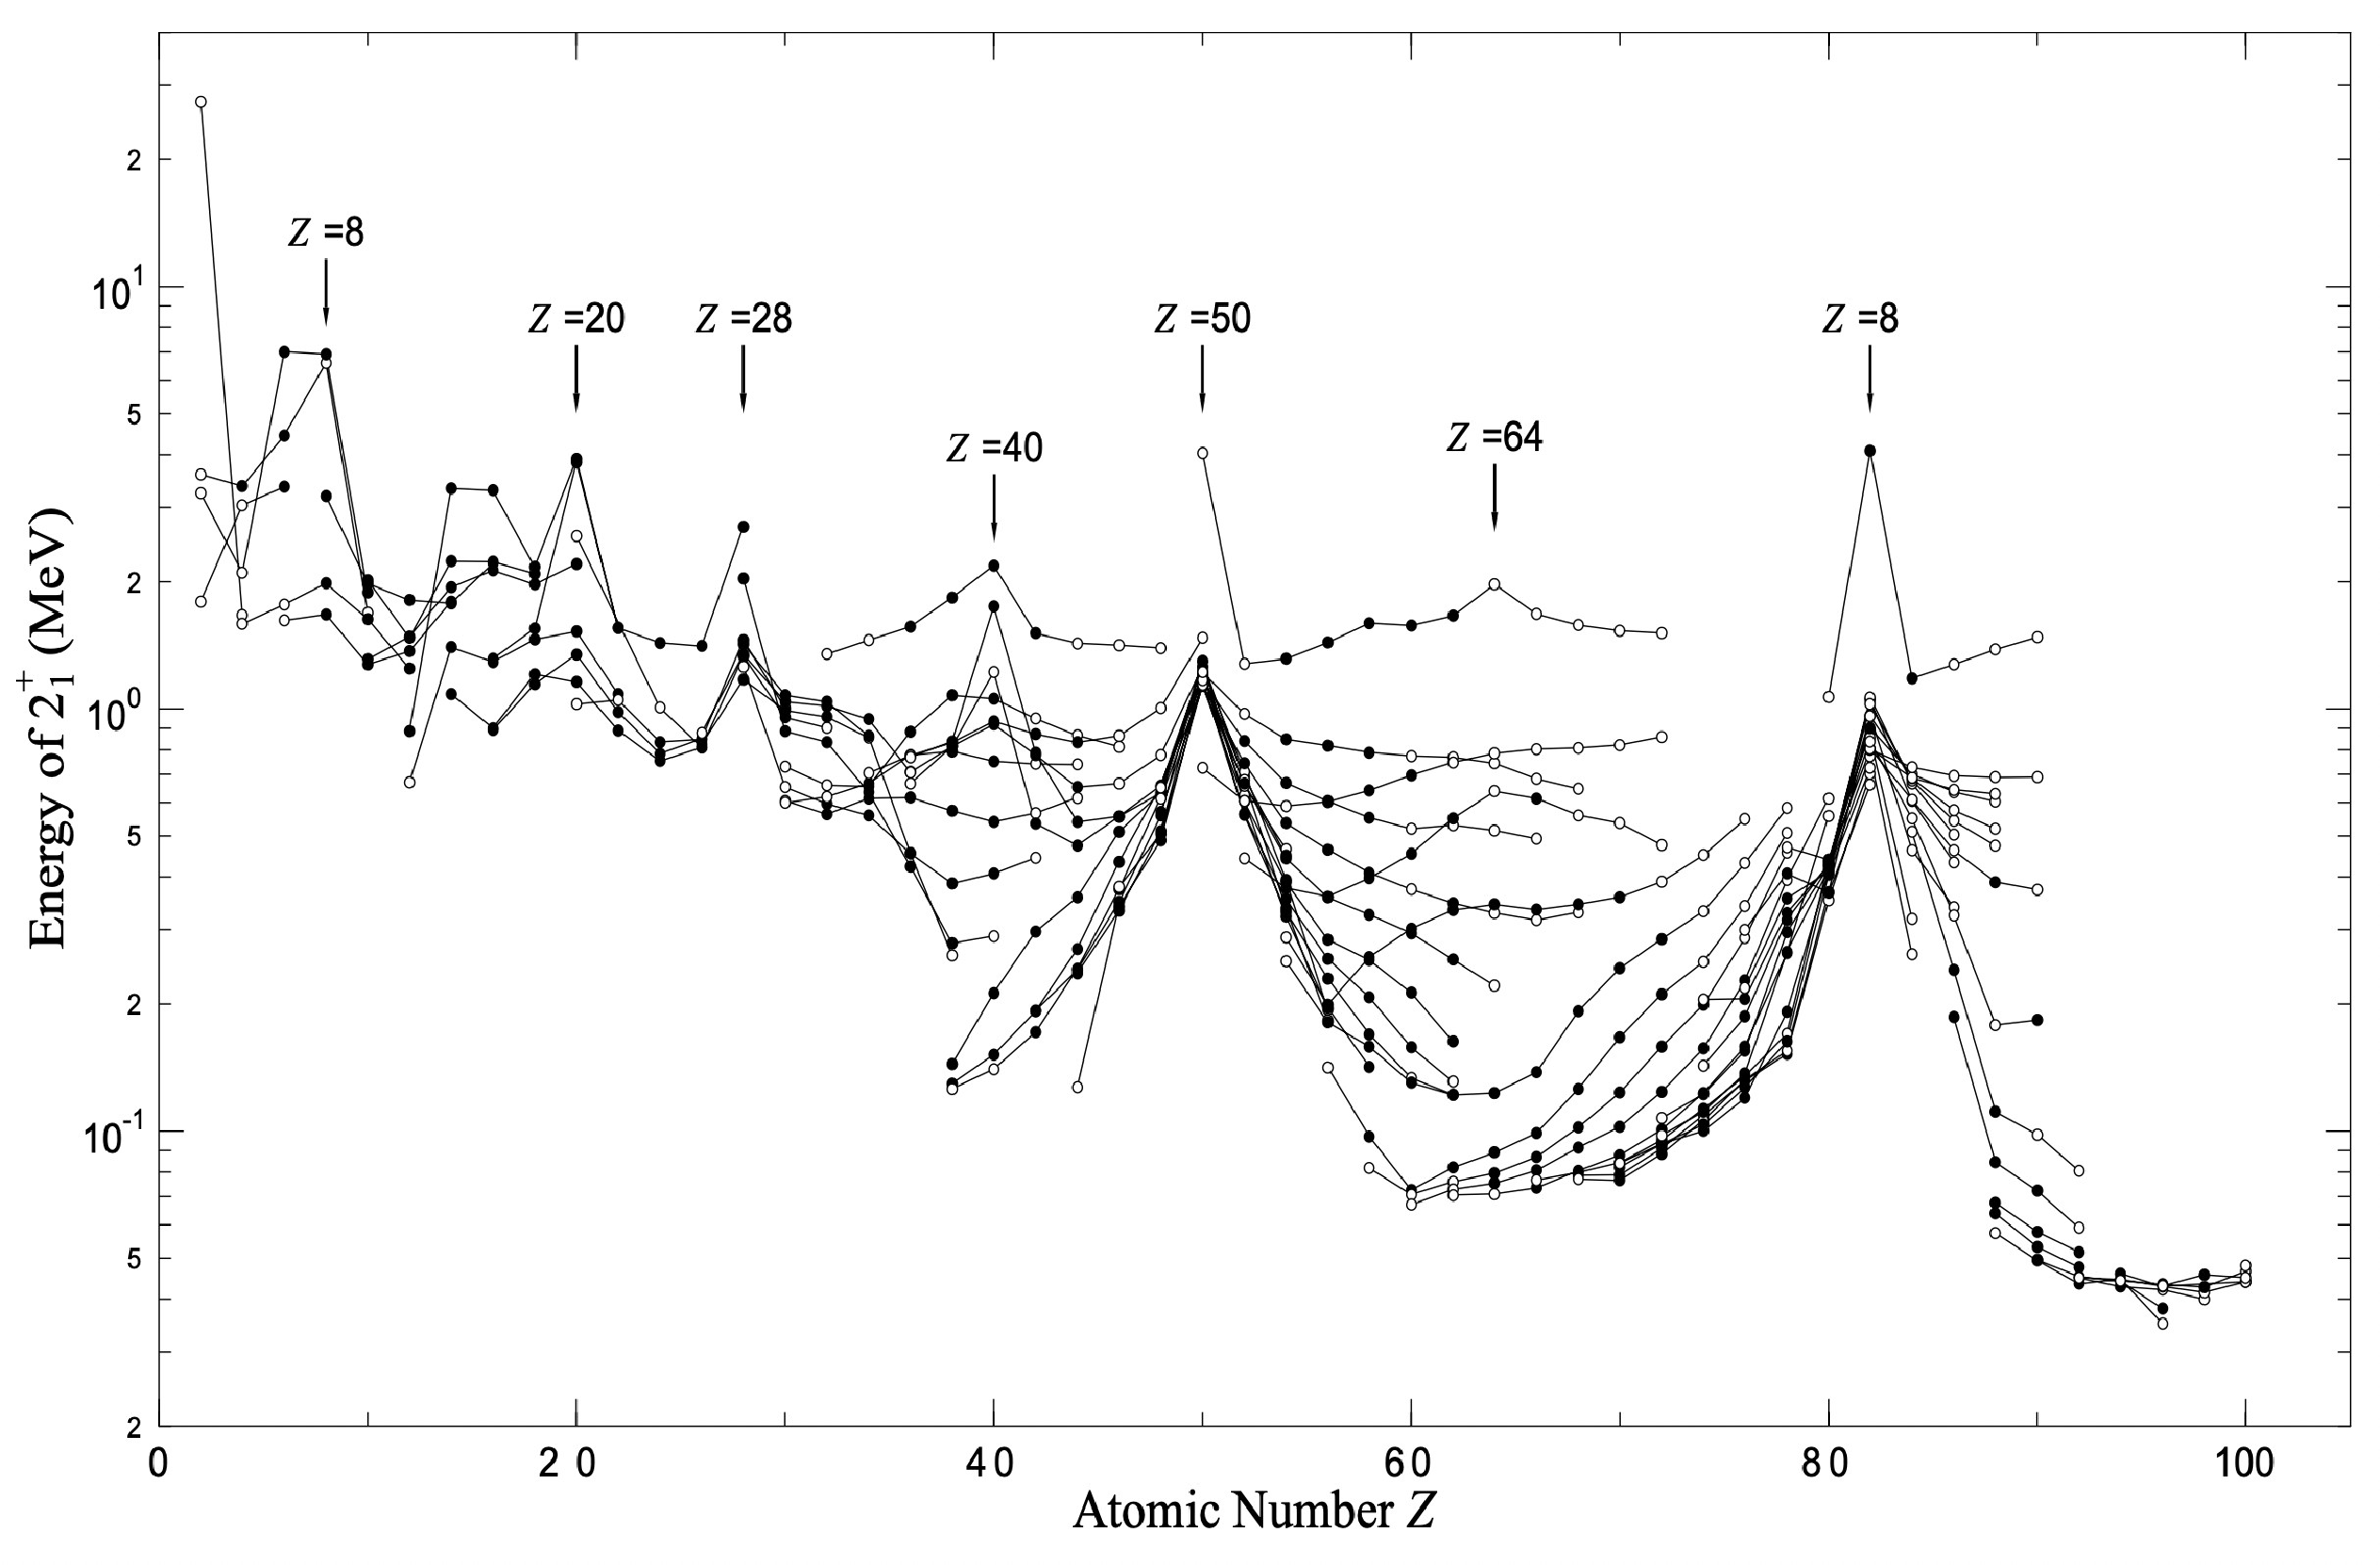
\includegraphics[width=0.99\textwidth]{Chapters/Figures/E2plus_proton.pdf}
    \caption{The first excited energy states $2^+$ of nuclei with even $Z$ and $N$ are graphically represented with respect to the proton number. Each connecting line represents a set of isotopes. Figure taken from Ref. \cite{matta2017exotic}.}
    \label{e2plus_proton}
\end{figure}
\begin{figure}
    \centering
    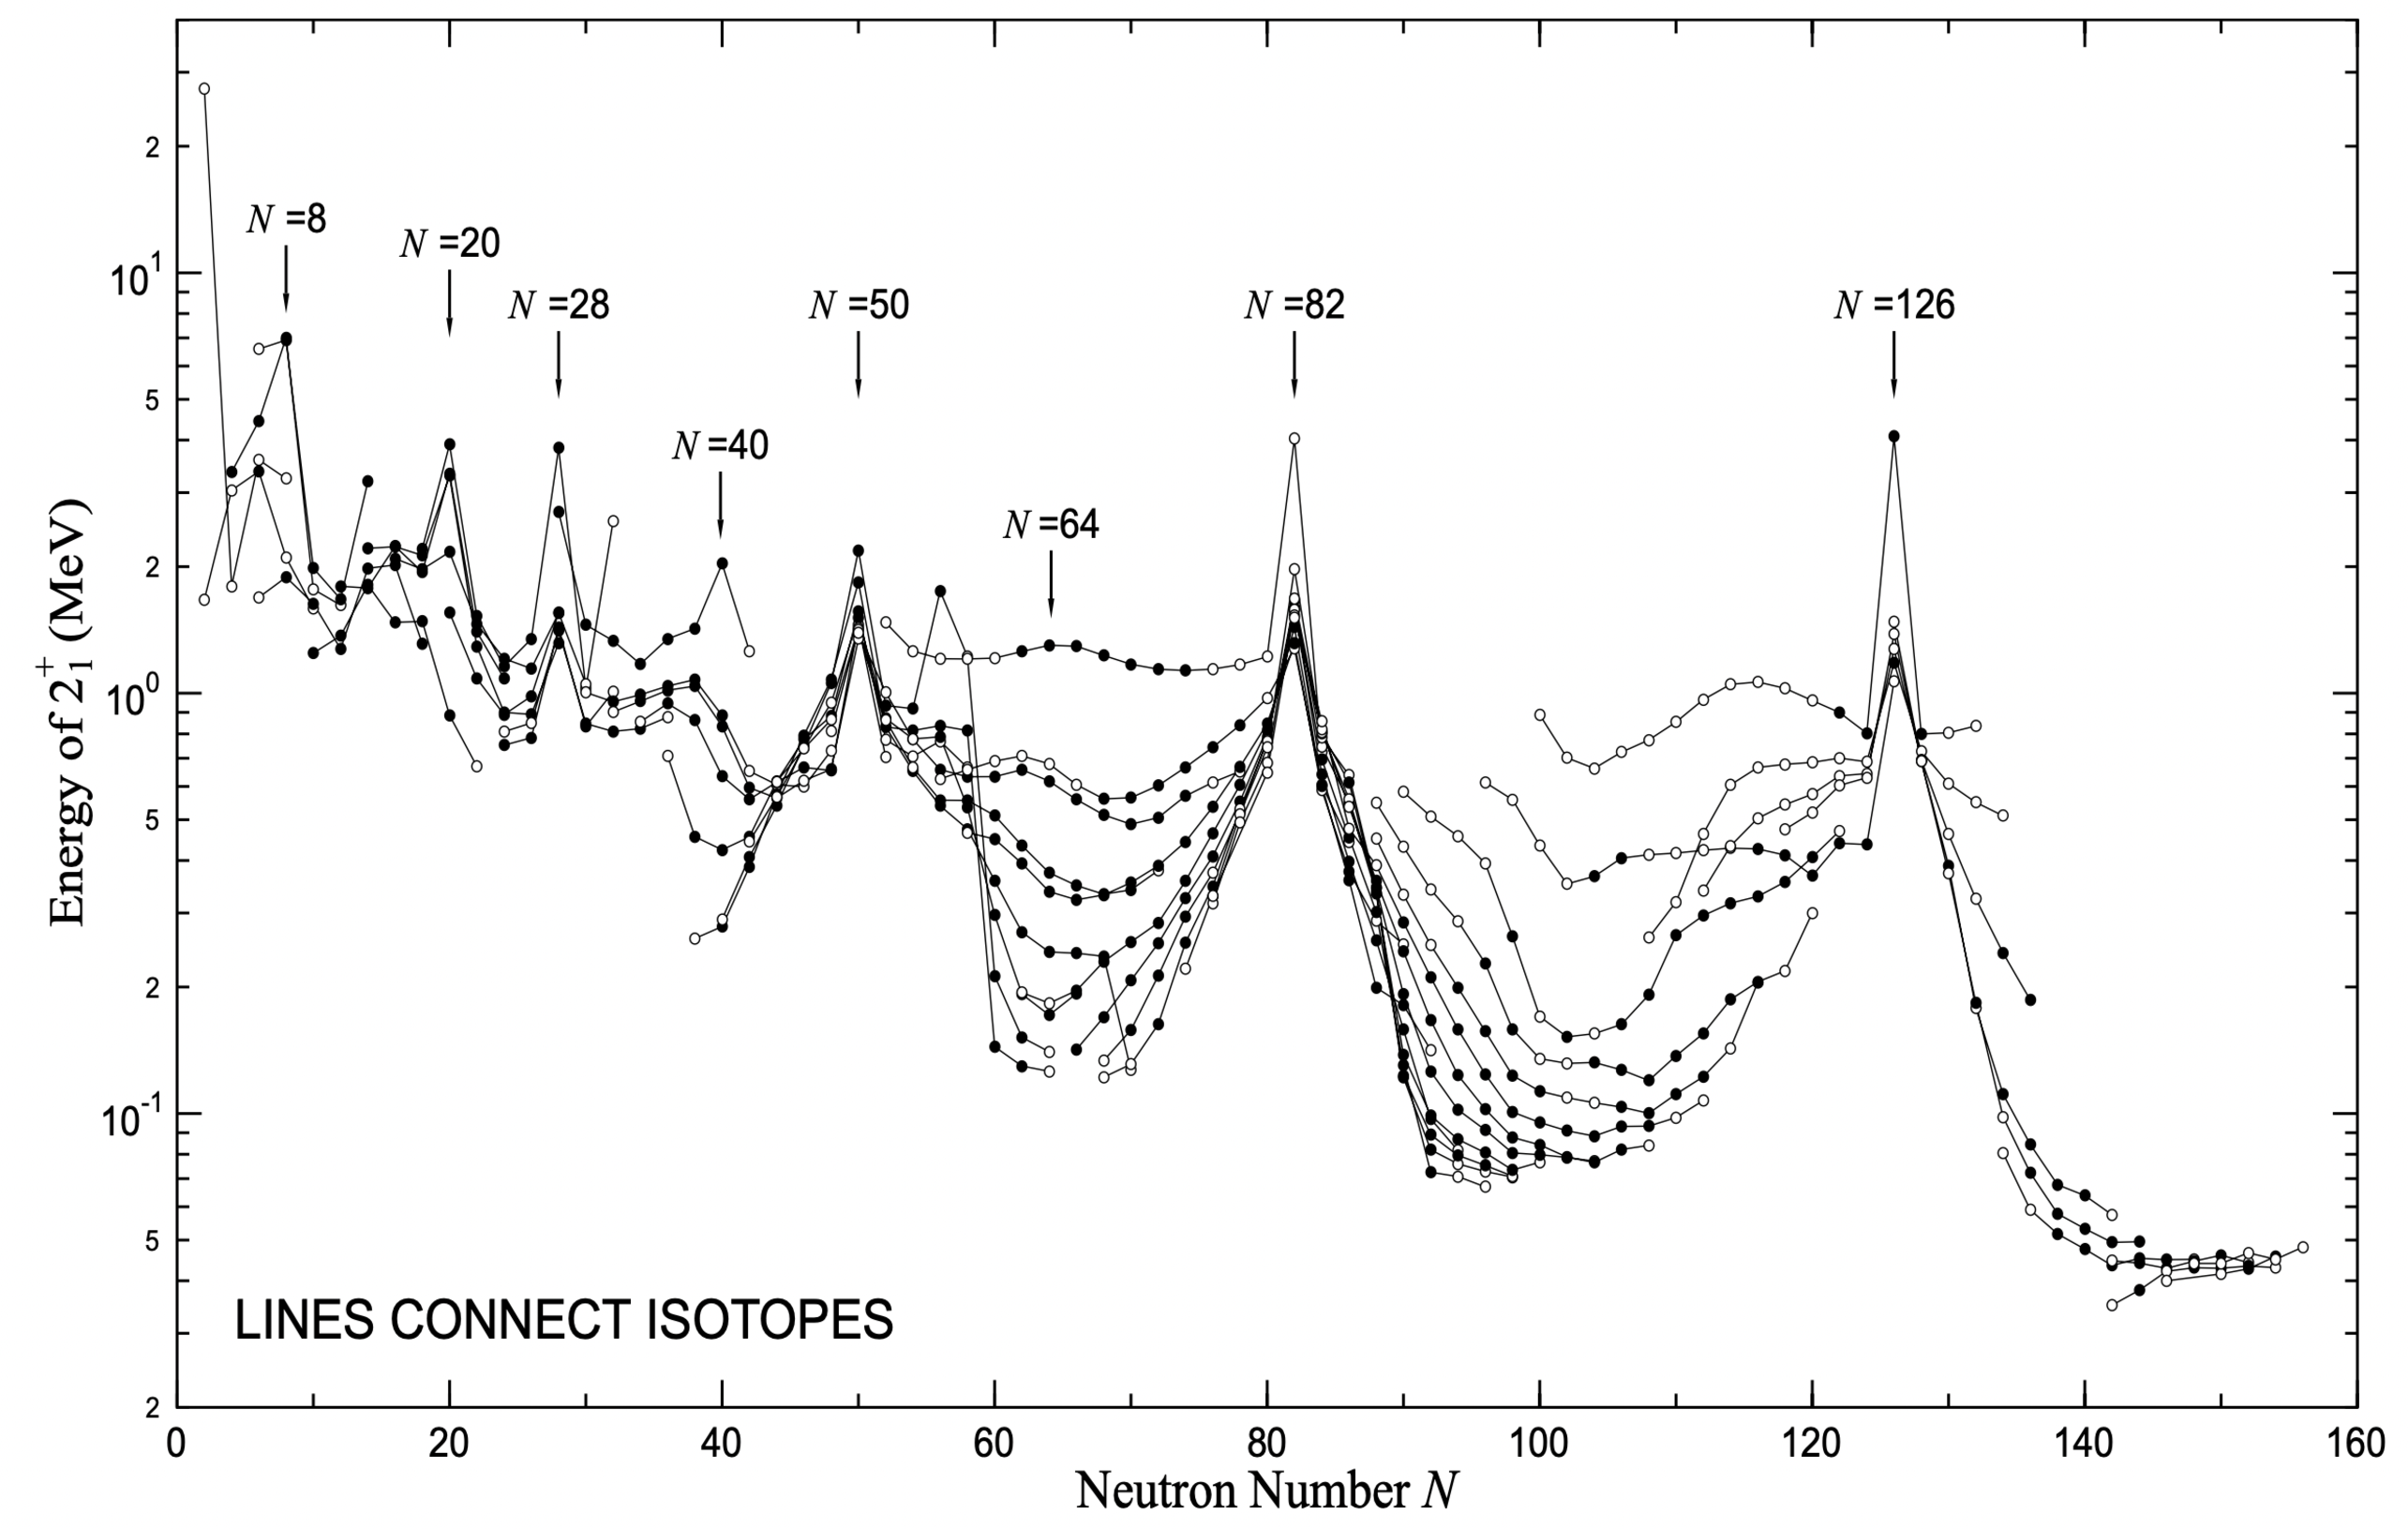
\includegraphics[width=0.99\textwidth]{Chapters/Figures/E2plus_neutron.pdf}
    \caption{The first excited energy states $2^+$ of nuclei with even $Z$ and $N$ are graphically represented with respect to the neutron number. Each connecting line represents a set of isotopes. Figure taken from Ref. \cite{matta2017exotic}.}
    \label{e2plus_neutron}
\end{figure}

The shell model starts from the basic assumption that the nucleus is a \emph{mean-field potential}, where the motion of a single nucleon is caused by all the other nucleons. In other words, the nucleon is moving inside an average potential generated by all the other constituents of the nucleus. Of course that all the nucleons under the influence of this mean field occupy the energy levels which correspond to a series of sub-shells verifying the \textit{Pauli exclusion principle}. Having a general expression for the potential that reproduces all the magic numbers and the observed nuclear properties is therefore crucial. Since the model starts from the concept of independent (non-interacting) particle motion within an average potential, finding each energy will be equivalent of solving the Schrödinger equation:
\begin{align}
    -\frac{\hbar^2}{2m}\nabla ^2\psi_i(r)+V(r)\psi_i(r)=e_i\psi_i(r)\, 
    \label{schrodinger-single-particle-eq}
\end{align}
where $e_i$ represents the energy (eigenvalue), $\psi_i$ represents the wave-function (eigenstates), and $V(r)$ is the nuclear potential whose expression must be evaluated. The choice of $V(r)$ will be dictated by the reproduction of various experimental data (such as nuclear saturation, scattering, nuclear reactions, and so on). For the motion of an independent particle, an obvious first attempt would be the \emph{simple harmonic oscillator} (SHO), which has the known expression:
\begin{align}
    V(r)=\frac{1}{2}m(\omega_i r)^2\ ,
    \label{harmonic-potential}
\end{align}
with $\omega_i$ as the frequency of the basic harmonic-like motion of the particle in the nucleus. With Eq. \eqref{harmonic-potential}, the motion of the nucleon has a straightforward expression:
\begin{align}
    \frac{\hbar^2}{2m}\nabla^2\psi_i(r)+\frac{1}{2}m(\omega r)^2\psi_i(r)=e_i\psi_i(r)\ .
\end{align}

This Schrödinger equation has its energy eigenvalues under to form:
\begin{align}
    e_N=\left(N+\frac{3}{2}\right)\hbar\omega\ ,
\end{align}
where $N$ is the number of oscillator quanta which describes each major shell (also called the \emph{principal quantum number}). One should keep in mind that such an expression is typical for a three-dimensional and isotropic harmonic oscillator. The principal quantum number $N$ is furthermore defined as:
\begin{align}
    N=2(n-1)+l\ ,
\end{align}
with $n$ and $l$ being the \emph{radial} quantum number and \emph{orbital angular momentum} quantum number, respectively, taking values $n=1,2,3,\dots$ and $l=0,1,2,\dots,n-1$. In this first approximation, all the levels with the same principal quantum number $N$ are \emph{degenerate}, with a maximal degeneracy given by $2(2l+1)$. However, by using only the SHO term as the expression of $V(r)$, only the first three magic numbers are reproduced, meaning that some additional term(s) might be needed in order to consistently obtain the series of magic numbers.

Furthermore, the steepness of the SHO can be corrected with an \emph{attractive} term proportional to $l$-squared. This acts as a centrifugal term which provides an angular momentum barrier, lifting the degeneracy between the levels with the same principal quantum number $N$ and different values for the orbital angular momentum $l$. This SHO+$l^2$ adjustment is still not enough, such that a so-called \emph{spin-orbit} coupling term of the form $\vec{l}\cdot\vec{s}$ must be also added. This term comes from the consideration that the nucleon-nucleon interaction has a spin dependence, and the potential depends on the intrinsic spin $s$ ($\vec{s}$) and the orbital angular momentum $l$ ($\vec{l}$) of a nucleon. Since $\vec{j}=\vec{l}+\vec{s}$, two possible states emerge from a single value of $l$ (depending on wether $\vec{s}$ is parallel or anti-parallel to $\vec{l}$). The final will consist of the \emph{Modified Harmonic Oscillator} (MHO).
\begin{align}
    V(r)=\frac{1}{2}(\omega r)^2+B\ \vec{l}^2+A\ \vec{l}\cdot\vec{s}\ .
    \label{modified-harmonic-oscillator-eq}
\end{align}

For the sake of simplicity, the centrifugal term will be denoted within formulas without the vector symbol. Since the intrinsic spin of a nucleon is $s=1/2$, for a given value of $l$, there can be two values for the \emph{total angular momentum} (a.m.) $j=l\pm1/2$: one for each spin orientation with respect to the direction of the orbital a.m. Moreover, for every value of $l=0,1,2,3,4,\dots$, there is a similar notation $l=s,p,d,f,g,\dots$, respectively. Regarding the spectroscopic notation, usually, the value of $j$ is considered as a subscript; $nl_j$ (for example $1p_{1/2}$ and $1p_{3/2}$). For high enough shells, there can be splittings between $j+1/2$ and $j-1/2$ that are large enough to lower the $j+1/2$ state from one oscillator shell $n$ to one located below $n-1$. These types of levels are called \emph{intruder states}, and they have opposite parity $\pi=(-1)^l$ with respect to the shell that these levels will occupy.

Going back to the expression of the $\vec{l}\cdot\vec{s}$ term from Eq. \eqref{modified-harmonic-oscillator-eq} and denoting it with $V_{ls}(r)$, its contribution to the total potential can be regarded as a surface effect and it can be expressed as a function that depends on the radial coordinate as such \cite{casten2000nuclear}:
\begin{align}
    V_{ls}(r)=-a_{ls}\frac{\partial V(r)}{\partial r}\vec{l}\cdot\vec{s}\ ,
\end{align}
where $V(r)$ is the expression for a central potential and $a_{ls}$ is a strength constant.

The nuclear potential is now able to reproduce all the magic numbers. It is also possible to formulate the total energy of a single-particle within the average potential. Thus, the Hamiltonian of this simple system (i.e., the MHO) can be formulated as such:
\begin{align}
    H&=-\frac{\hbar^2}{2m}\nabla^2+V_\text{SHO}+(l^2)_\text{term}+(\vec{l}\cdot\vec{s})_\text{term}=-\frac{\hbar^2}{2m}\nabla^2+V_\text{MHO} , \nonumber\\
    H&=-\frac{\hbar^2}{2m}\nabla^2+\frac{1}{2}m(\omega r)^2+Bl^2+A\vec{l}\cdot\vec{s}\ .
\end{align}

The evolution from a SHO, then SHO+$l^2$, and finally SHO+$l^2+\vec{l}\cdot\vec{s}$ or modified oscillator potential is illustrated in Fig. \ref{energy-levels-mho}, where it can be seen how each extra term removes a degeneracy, with the complete reproduction of the magic numbers in the third column. The \emph{intruder} levels can also be observed, where states with $j=l+1/2$ from a particular $n$ are so low, that they lie below an $n-1$ adjacent level.
\begin{figure}
    \centering
    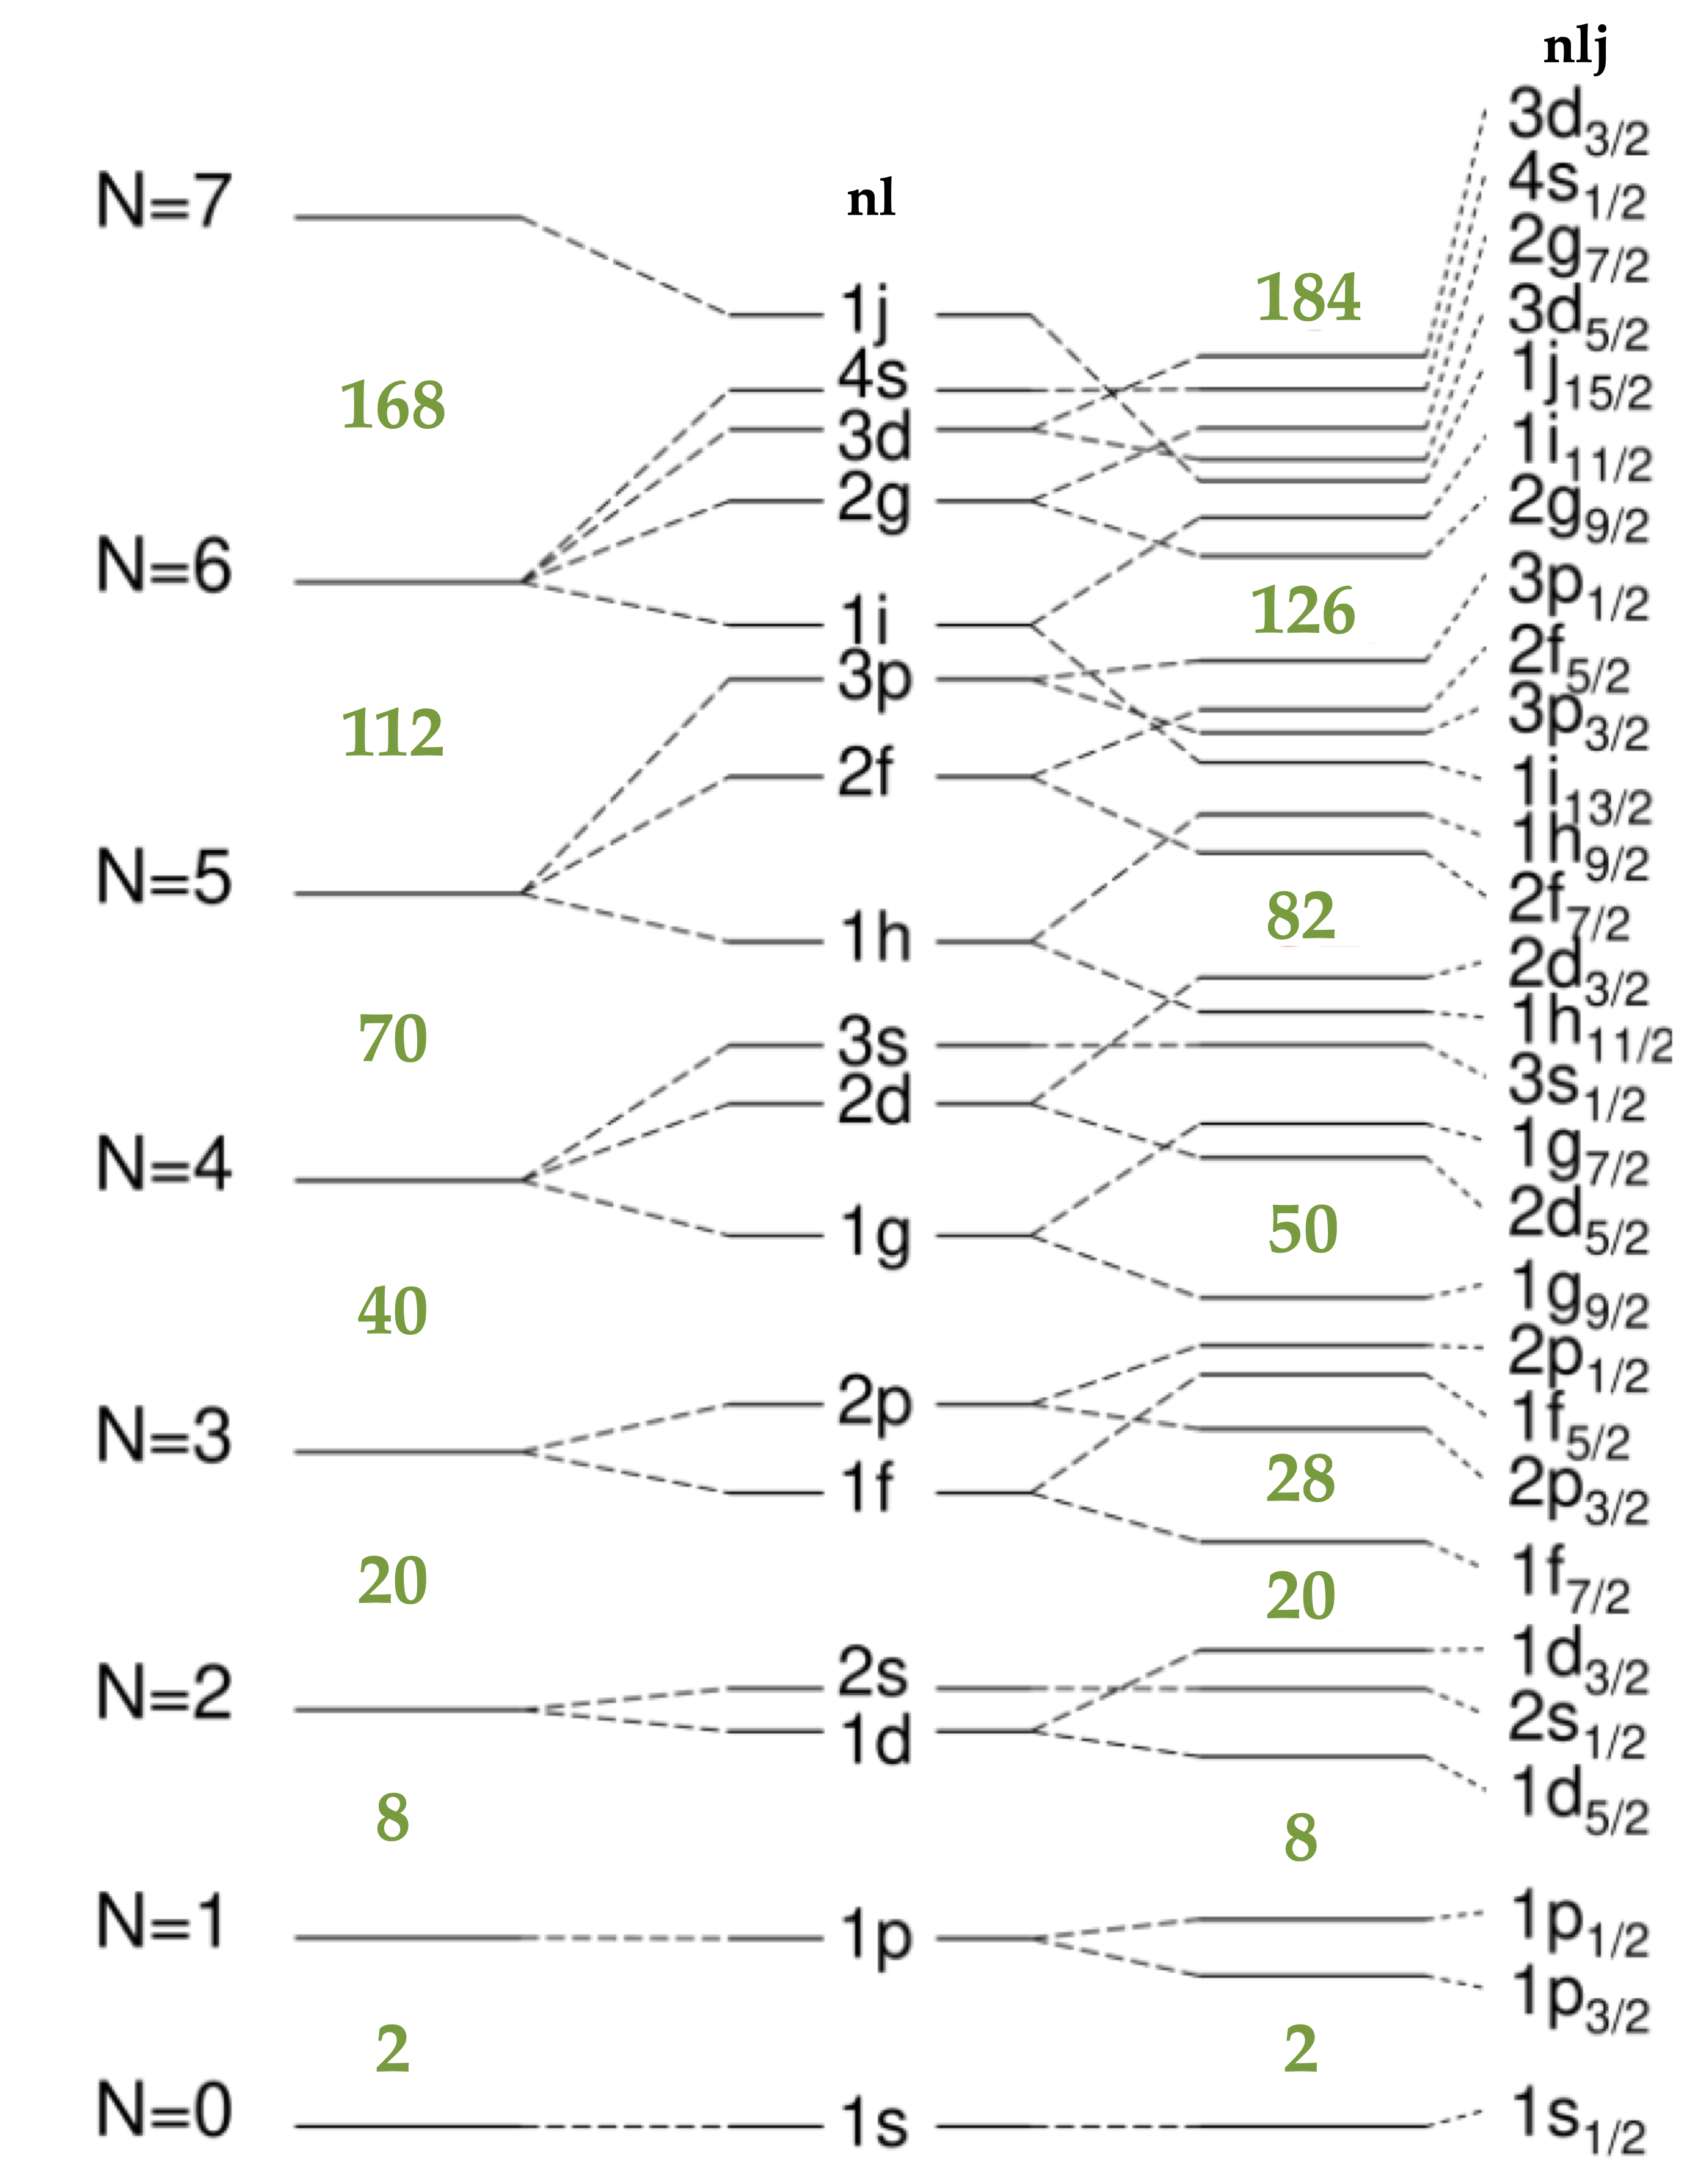
\includegraphics[width=0.99\textwidth]{Chapters/Figures/SM_level_scheme.png}
    \caption{The energy levels obtained via calculation of the shell model potential using the simple oscillator (SHO), the SHO amended with a centrifugal term $l^2$, and finally the modified oscillator (MHO) that contains a spin-orbit term. The `correct' magic numbers are the ones in the right-most column. Figure is adapted from Refs. \cite{krane1991introductory,matta2017exotic}.}
    \label{energy-levels-mho}
\end{figure}

Another, more realistic potential that can be used in order to reproduce the specific shell model calculation is the so-called Woods-Saxon potential. Because of the short-range character of the strong nuclear force, it is safe to assume that this potential should behave in the same manner as the density distribution of the nucleons. Since for medium and heavy nuclei, the Fermi-like functions (distributions) are the ones that best fit the experimentally measured data, this potential should have the following form \cite{woods1954diffuse}:
\begin{align}
    V_\text{ws}(r)=-\frac{V_0}{1+e^{\frac{r-R_0}{a}}}\ ,
    \label{woods-saxon-potential}
\end{align}
where $V_0$ represents the depth of the potential ($\approx 50$ MeV, in order to reproduce the experimental separation energies for the nucleons), $a$ is the surface thickness (or \emph{diffuseness parameter}, giving information about how fast the potential drops to zero) with a value of approximately $0.5$ fm, and $R_0$ is the nuclear radius ($R_0=1.2A^{1/3}\ \text{fm}$). The nature of this potential is of \emph{central type} and Eq. \eqref{woods-saxon-potential} is not enough the reproduce the higher magic numbers. As such, the addition of a spin-orbit term, similarly as in the case of MHO potential, is required \cite{martin2017particle}: 
\begin{align}
    V_\text{total}=V_\text{ws}^\text{central}+V_{ls}(r)\vec{l}\cdot\vec{s}\ .
    \label{woods-saxon-so-potential}
\end{align}
The only good quantum numbers in the case of the WS potential are the total a.m. $j$ and the parity $\pi=(-1)^l$.
The expectation value of the spin-orbit term $\vec{l}\cdot\vec{s}$ can be given as:
\begin{align}
    \langle ls \rangle=\hbar^2\begin{cases}
        \frac{l}{2} \quad &\text{for} j=l+\frac{1}{2}\\
        -\frac{l+1}{2} &\text{for} j=l-\frac{1}{2}\ \\
    \end{cases}\ .
\end{align}
and the spacing between two levels can be furthermore expressed as \cite{martin2017particle}:
\begin{align}
    \Delta E_{ls}=\frac{2l+1}{2}\hbar^2\langle V_{ls}\rangle\ .
\end{align}
The experimental evidence points to the fact that $V_{ls}(r)$ is negative, meaning that states with $j=l-1/2$ are shifted higher than $j=l+1/2$. Some characteristics of the WS potential are the following:
\begin{enumerate}
    \item It increases with the increase of $R$, meaning that it has an \emph{attractive nature}
    \item It flattens out for large enough $A$ in the center of the nucleus
    \item It rapidly goes to zero as $R$ increases (given by the diffuseness parameter), indicating its short-range nature
    \item When $R=R_0$ (that is for the nucleons near the surface), a large force towards the center of the nucleus is experienced by the these nucleons.
\end{enumerate}
\begin{figure}
    \centering
    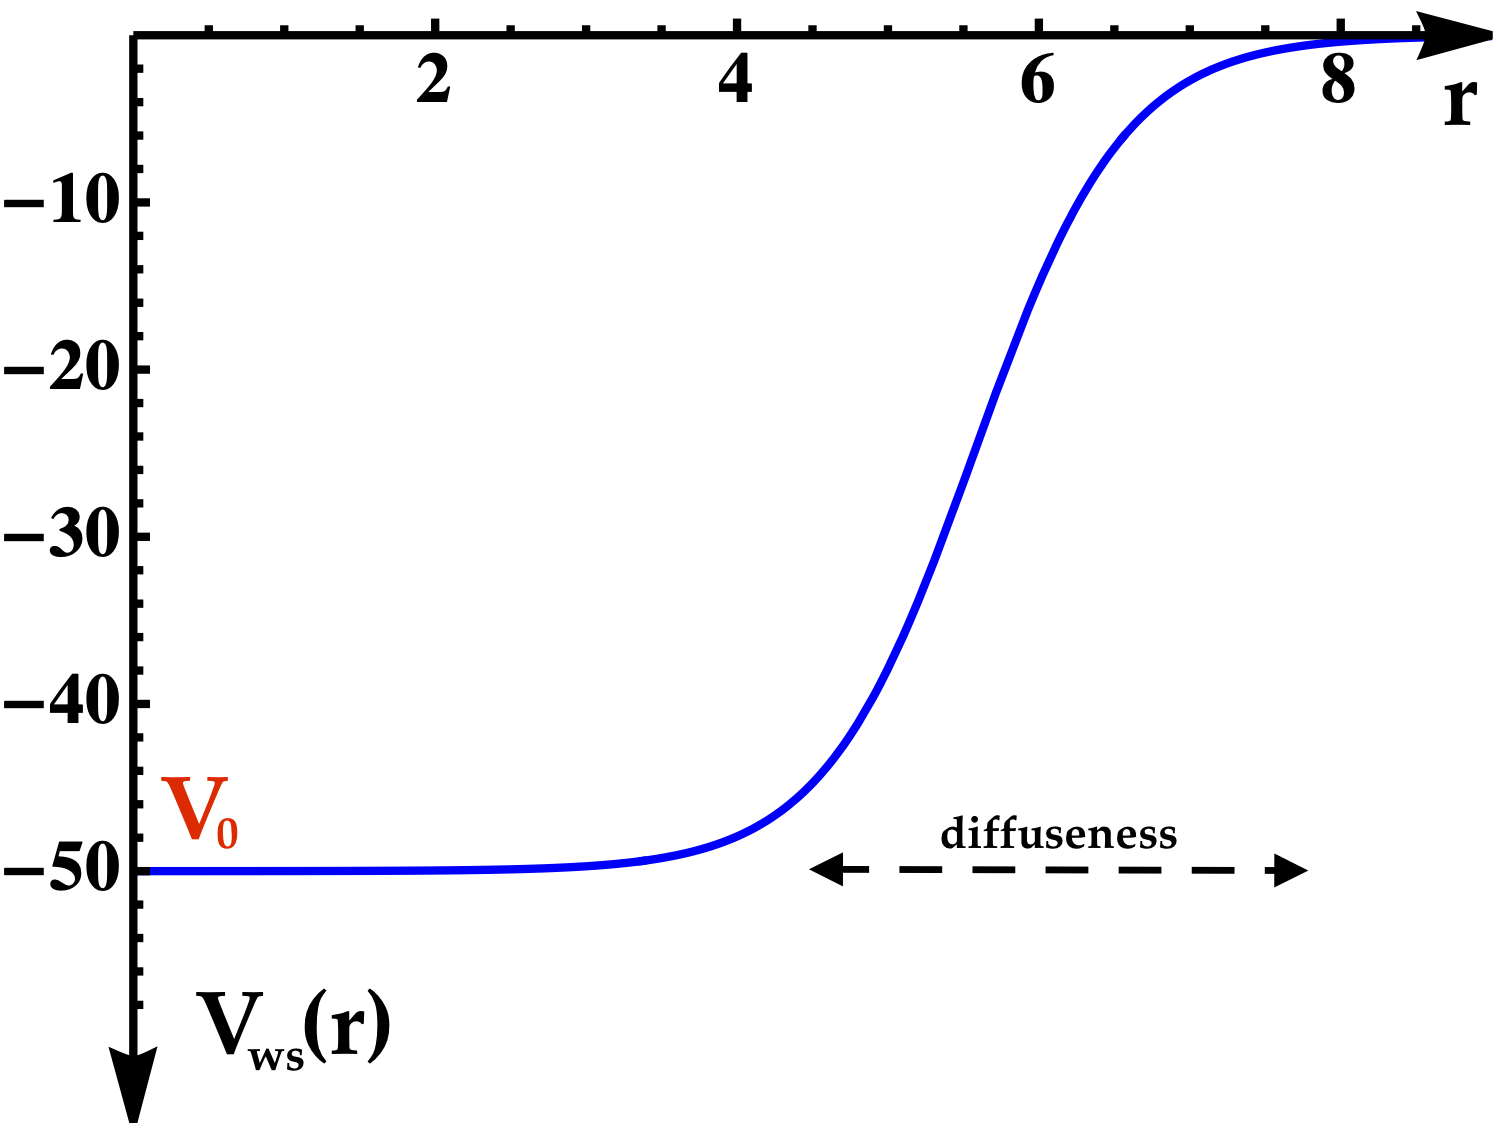
\includegraphics[scale=0.2]{Chapters/Figures/ws_potential_plot.png}
    \caption{The shape of the Woods-Saxon potential, defined by Eq. \eqref{woods-saxon-potential}. The parameters are arbitrarily chosen as: $V_0=50$ MeV, $R=5.57$ fm, and $a=0.5$ fm.}
    \label{woods-saxon-plot}
\end{figure}

The Hamiltonian that describes the motion of the nucleon within the mean-field potential is given by:
\begin{align}
    %H&=-\frac{\hbar^2}{2m}\nabla^2+V_\text{ws}^\text{central}+(\vec{l}\cdot\vec{s})_\text{term}\ ,\\
    H&=-\frac{\hbar^2}{2m}\nabla^2-\frac{V_0}{1+e^{\frac{r-R_0}{a}}}+A\vec{l}\cdot\vec{s}\ ,
\end{align}
and the shape of a typical Woods-Saxon potential is shown in Fig. \ref{woods-saxon-plot}. A comparison between the Woods-Saxon potential, a SHO, and the square-well-like potential is made in Fig \ref{shell-model-functional-potentials}. The difference between the pure form of the Woods-Saxon potential and the total potential amended with the spin-orbit contribution can be seen in Fig. \ref{woods-saxon-energy-levels}.
\begin{figure}
    \centering
    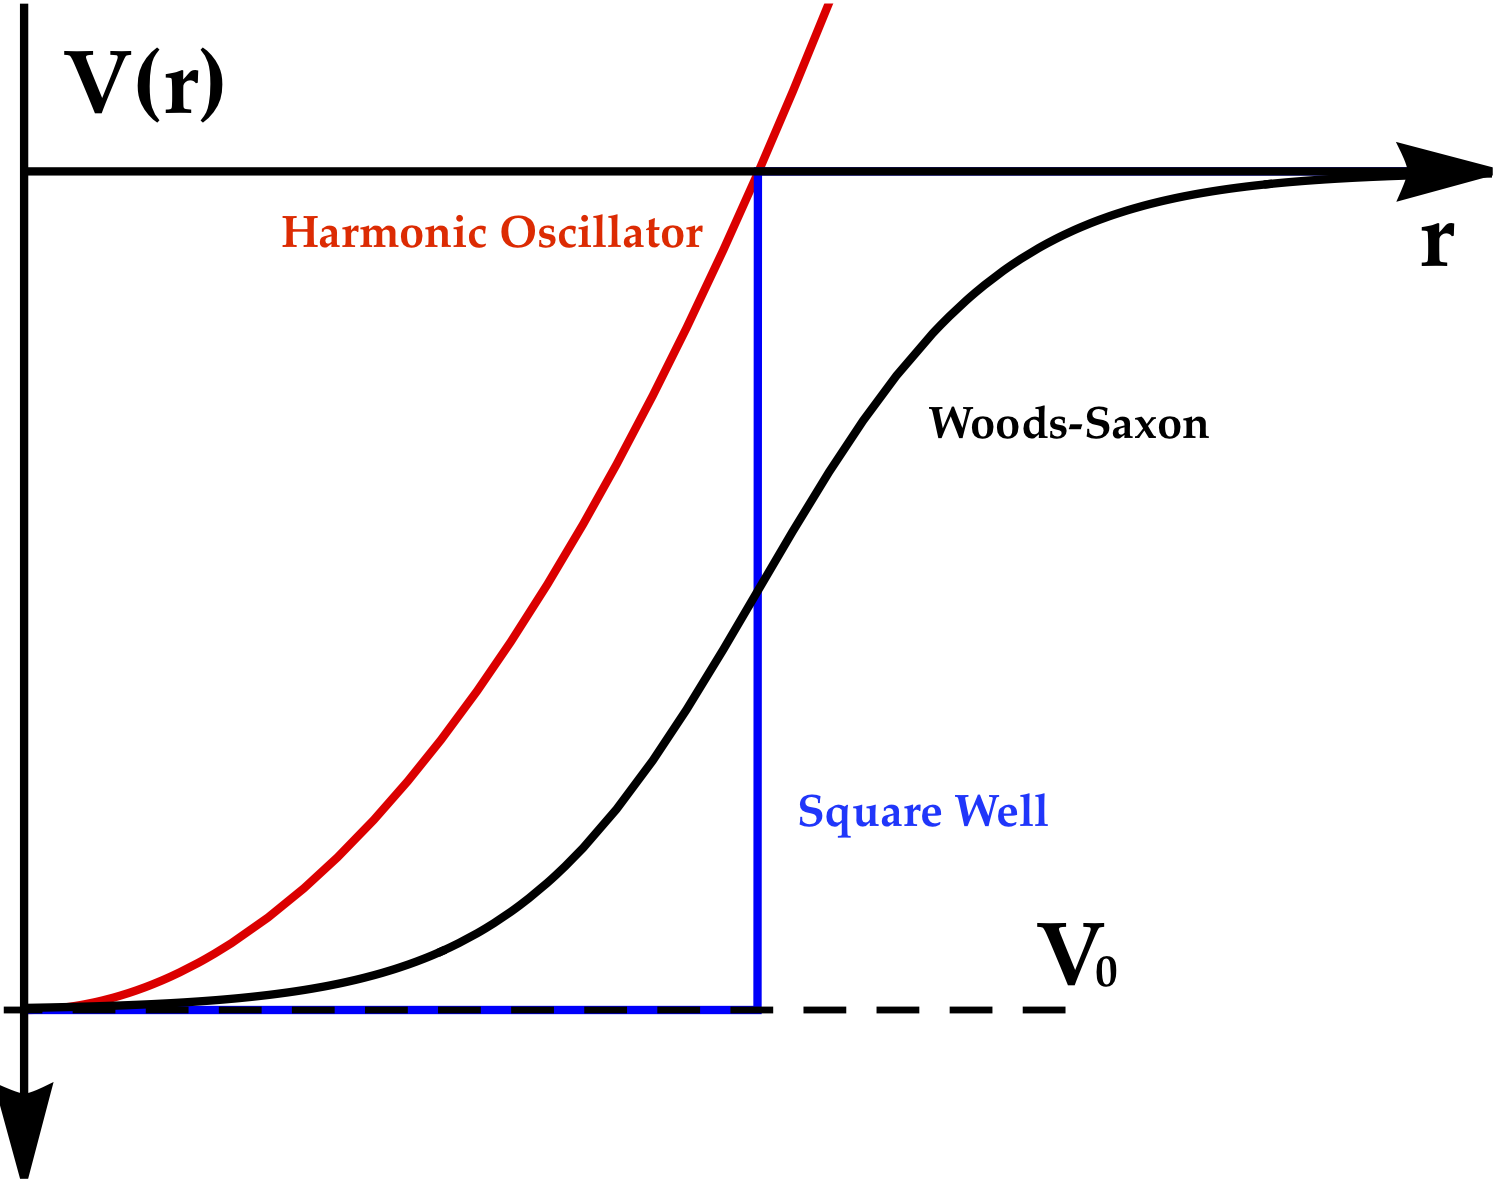
\includegraphics[scale=0.2]{Chapters/Figures/functional-potentials-shell-model.png}
    \caption{A schematic representation with the three kind of potentials used to describe the shell model: harmonic oscillator, Woods-Saxon, and for completeness, the square-well.}
    \label{shell-model-functional-potentials}
\end{figure}
\begin{figure}
    \centering
    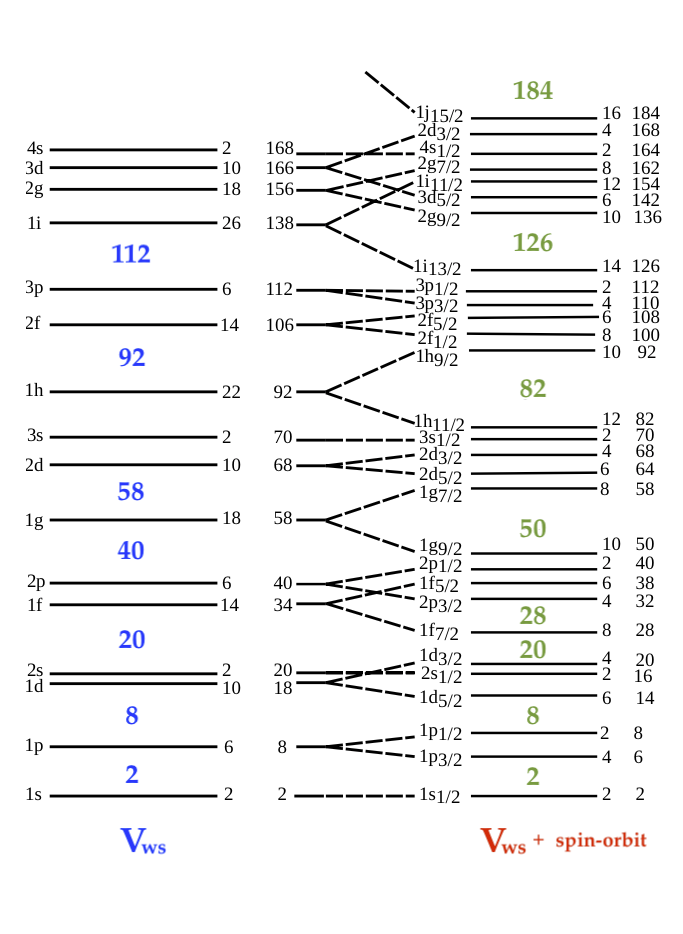
\includegraphics[width=0.99\textwidth]{Chapters/Figures/energy_levels_WS.png}
    \caption{The energy levels calculated for the Woods-Saxon potential given by Eq. \eqref{woods-saxon-potential} (left-side), and the single-particle energies with the spin-orbit correction added, as in Eq. \eqref{woods-saxon-so-potential} (right-side). Figure adapted from Ref. \cite{lewis2019lifetime}.}
    \label{woods-saxon-energy-levels}
\end{figure}

So far, the general discussion concerning nuclear models was made for the case where each nucleon is treated as an \emph{independent} particle moving in an average (mean-field) potential. However, such an assumption is not accurate enough (especially for the nuclei that lie far away from the closed shells), and this problem should be treated within a \emph{many-body} approach: considering the mutual interaction between the nucleons. These interactions are also called \emph{residual interactions} \cite{casten2000nuclear,bertulani2007nuclear}. With these residual interactions, an accurate depiction of the nucleus might be achieved. The \emph{Deformed Shell Model} will be employed in the following sections, reaching to the famous Nilsson model of describing the nucleus.

\section{Nilsson Orbitals}
\label{appendix:extra-nilsson-orbitals}

Recalling Fig. \ref{nillson-orbits-splittings}, the splitting of an orbital into $j+1/2$ magnetic sub-states can be viewed as a set of energies where the nucleon is \emph{orbiting} around the bulk nucleus with an orbit that has a certain \emph{tilt} angle $\theta$ (see the orbits depicted in Figs. \ref{nillson-orbits-prolate-projections} - \ref{nillson-orbits-oblate-projections}). The tilting angle is conceptually shown in Fig. \ref{fig-nilsson-tilting-angle}. For that particular orbit, the angle is given by the expression \cite{krane1991introductory,casten2000nuclear}:
\begin{align}
    \sin\theta&=\frac{\Omega}{j}\ , \nonumber\\
    \theta&=\arcsin(\frac{\Omega}{j})\ .
    \label{theta-tilting-angle}
\end{align}
\begin{figure}
    \centering
    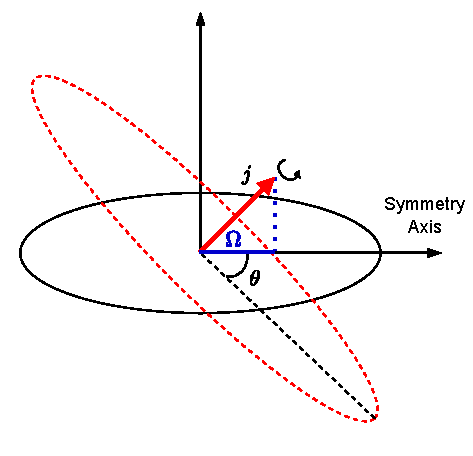
\includegraphics[scale=1]{Chapters/Figures/nilsson_tilting_angle.pdf}
    \caption{The orbit of a single particle orbiting the deformed nucleus, defined by the projection of the particle's a.m. $\Omega$ (on the symmetry axis) and the tilting angle $\theta$. Figure inspired from Ref. \cite{casten2000nuclear}}
    \label{fig-nilsson-tilting-angle}
\end{figure}

The change of $\theta$ is rather slow for low $\Omega$ projections, while rapid changes take place at high $\Omega$ values. %It should be noted that this discussion applies to a single-particle total a.m. projection, but as it was discussed previously, using the projection $K$ within calculations is equivalent (since the axially deformed potentials keep $\mathbf{R}$ oriented perpendicular to the symmetry axis).
As a numerical example, the $\theta$ variation is studied for the orbits $j=\{9/2,11/2,13/2\}$, with their corresponding projections. The evolution with $\Omega$ for different orbits can be seen in Fig. \ref{fig-tilting-angle-shape}.
\begin{figure}
    \centering
    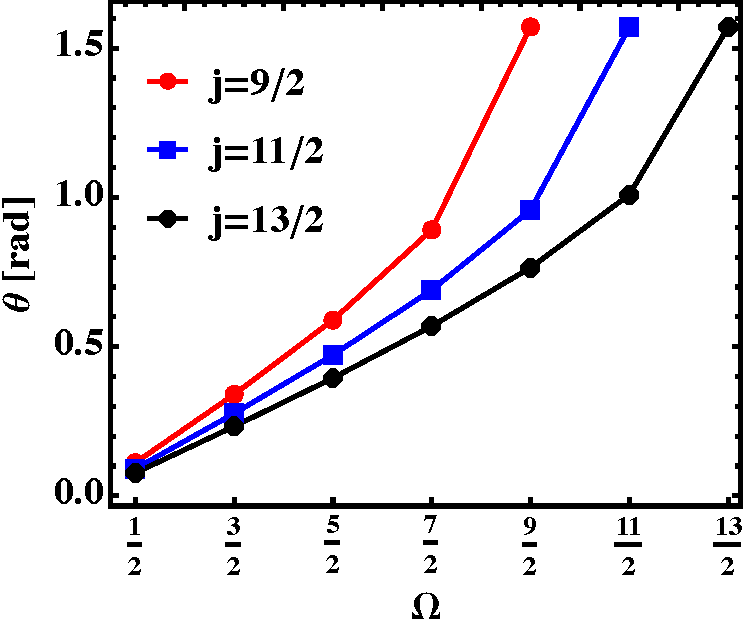
\includegraphics[scale=0.7]{Chapters/Figures/tilted_theta_shape.pdf}
    \caption{The change in $\theta$ angle defined in Eq. \eqref{theta-tilting-angle} with increasing values of $\Omega$, for a few orbitals $j$.}
    \label{fig-tilting-angle-shape}
\end{figure}

The splitting of an orbital $j$ into multiple sub-states (see Fig. \ref{nillson-orbits-splittings}) emerges from the considerations regarding the change in tilting angle and also the fact that the difference in energy is rather smooth (high) depending on low (high) $\Omega$ values. Based on this discussion, it is clear that a full Nilsson diagrams is constructed with the configuration mixing of different $j$ values.
% The configuration is superimposed on state-splitting via the $\Omega$ projections. With this idea, one can state that
Remarkable, \emph{no two lines in the Nilsson diagram with similar $\Omega$ values can cross each other}. When two such orbits come close to each other, they must repel as shown in Fig. \ref{fig-non-crossing}. Explaining the behavior of the lines that appear in the Nilsson diagrams \ref{nillson-diagram} - \ref{nillson-diagram-2} is straightforward: each line represents a Nilsson state, starting out straight and then sloping downward or upward, depending on the angle of the orbit relative to the bulk nucleus. The \emph{curving} of an orbit starts when it approaches another level with the same quantum number $\Omega$ and parity $\pi$. Thus, the structure of any Nilsson diagram relies on three main features \cite{casten2000nuclear}:
\begin{itemize}
    \item the $\Omega$ splitting
    \item repulsion between two levels
    \item single-particle shell model energies
\end{itemize}

Taking a closer look at the Nilsson from Fig. \ref{nillson-diagram-2}, there are two orbits within the $82$-$126$ neutron gap that can be analyzed in terms of \emph{mixing}: $f_{7/2}$ and $h_{9/2}$, respectively. Obviously, the lack of deformation implies a degeneracy of these orbits, but when deformation occurs, splitting kicks in. The angle of the orbital orientation $\theta$ depends on the ratio $\Omega/j$ (recall $\theta=\arcsin(\Omega/j)\approx\Omega/j$ at low $\Omega$). Small tilting angles will occur due to i) small values of $\Omega$ or ii) high $j$. As a result, the energies for the orbits $\Omega=1/2,3/2,5/2$ belonging to the $h_{9/2}$ shell are decreasing in energy faster with deformation than those from $f_{7/2}$ orbit. Consequently, the different rates of decrease for the Nilsson energies will overcome any small spherical energy separation $f_{7/2}-h_{9/2}$, making the orbits with low $\Omega$ to approach each other, leading to a more pronounced mixing. However, as discussed in \ref{appendix:two-state}, two orbits defined by the same quantum numbers cannot cross, causing the apparition of an \emph{inflection point}. The points can be seen when looking at the $\Omega=5/2$ and $\Omega=7/2$ orbits, which correspond to $f_{7/2}$ and $h_{9/2}$.

% Lastly, an alternative form of the Nilsson Hamiltonian should be expressed, taking into consideration the already studied nuclear radius (see Eq. \eqref{nuclear-shape} which describes the shape of the nuclear surface) and the fact that until now, only the \emph{quadrupole} effects have been relevant to the discussion about deformed potentials in nuclei. Indeed, for quadrupole deformations, the nuclear radius can be simplified to:
% \begin{align}
%     R(\theta,\varphi)=R_0\left(1+\beta Y_2^0(\theta,\varphi)\right)\ .
%     \label{simple-quadrupole-nuclear-surface}
% \end{align}

The single-particle Hamiltonian can be written in the general form, starting from the expression Eq. \eqref{eq-full-nilsson-ham}:
\begin{align}
    H_\text{Nil}=-\frac{\hbar^2}{2m}+\frac{1}{2}m(\omega_0r)^2-&\frac{4}{3}\sqrt{\frac{\pi}{5}}m(\omega_0r)^2\epsilon Y_2^0(\theta,\varphi)-2\kappa\hbar\omega_0(\vec{l}\cdot\vec{s})\nonumber\\
    &-2\kappa\hbar\omega_0\mu\left(l^2-\langle l^2\rangle_N\right)\ .
    \label{eq-nilsson-ham-spherical-harmonics}
\end{align}

The expressions for the oscillator frequencies were already defined as functions of the deformation parameter $\epsilon$ and they keep the same form  as Eqs. \eqref{oscillator-frequencies-nilsson} - \eqref{omega-0-oscillator-frequency}. It is worth mentioning that both forms of $H_\text{Nil}$ from Eq. \eqref{eq-full-nilsson-ham} and Eq. \eqref{eq-nilsson-ham-spherical-harmonics} are equivalent. Moreover, they describe the structure of the deformed nuclei in the limits of large deformations (via Eq. \eqref{eq-full-nilsson-ham}) and small deformations (via Eq. \eqref{eq-nilsson-ham-spherical-harmonics}). Within literature, the two parameters are taken to be $\kappa\approx 0.06$ and $\mu$ varies between $\mu=0\sim 0.7$.% As previously shown, the relationship between the $\epsilon$ and $\beta$ deformation parameters is given by $\epsilon=\frac{3}{2}\sqrt{\frac{5}{4\pi}}\beta\approx 0.95\beta$.
% the formula for \epsilon nuclear deformation parameter is taken from Casten

When the deformations are small, $j$ is a good quantum number, and the Eq. \eqref{eq-nilsson-ham-spherical-harmonics} represents a Hamiltonian for the AHO plus a \emph{perturbation} that is proportional to $\epsilon r^2Y_2^0$. Therefore, one can consider the eigenstates of the Hamiltonian as states labelled by the quantum numbers $N$, $l$, $j$, and $m$. It is possible to obtain a shift in energies relative to $\epsilon=0$ if the angular part $Y_2^0$ is treated as a perturbation \cite{casten2000nuclear}:
\begin{align}
    \Delta E_{Nljm}=-\frac{4}{3}\sqrt{\frac{\pi}{5}}m\omega_2^0\epsilon\bra{Nljm}r^2Y_2^0\ket{Nljm}\ .
\end{align}

Furthermore, one can perform a separation of the radial and the angular parts while using the known relation for a harmonic oscillator potential:
\begin{align}
    \frac{1}{2}m\omega_0^2\bra{Nljm}r^2\ket{Nljm}=\frac{1}{2}\hbar\omega_0\left(N+\frac{3}{2}\right)\ ,
\end{align}
and together with the evaluation of the matrix elements for spherical harmonics, the final expression for the energy shift at small deformations is:
\begin{align}
    \Delta E_{Nljm}=-\frac{2}{3}\hbar\omega_0\left(N+\frac{2}{3}\right)\epsilon\frac{\left[3K^2-j(j+1)\right]\left[\frac{3}{4}-j(j+1)\right]}{(2j-1)j(j+1)(2j+1)}\ ,
    \label{nilsson-energy-shifts}
\end{align}
where the projection $m$ was replaced with the total angular momentum projection onto $z$-axis $K$. Based on Eq. \eqref{nilsson-energy-shifts}, the following properties for a Nilsson diagram emerge:
\begin{itemize}
    \item There is a $K^2$ dependence for the energy shifts
    \item The quadrupole deformation parameter ($\epsilon$ or $\beta$) shows a clear linear dependence for $\Delta E_{Nljm}$
    \item Another linear dependence for the shifts is induced by the principal (oscillator) quantum number $N$
    \item When the deformation parameter is positive, there are more downward sloping orbits than upward ones (example discussed below)
\end{itemize}

For a value $j>1/2$, the terms $\left[3K^2-j(j+1)\right]$ and $3/4-j(j+1)$ are negative, resulting in the following types of orbits: \cite{krane1991introductory}:
\begin{align}
    \text{downward sloping:}&\ K<\sqrt{\frac{j(j+1)}{3}}\approx\frac{j}{1.8}=0.57j\ ,\\
    \text{upward sloping:}&\ K>0.57j\ .
\end{align}

It was already shown that the angular orientation (i.e., the tilting angle $\theta$) of an orbit is given by $\theta=\arcsin(K/j)$. For a ratio $K/j=0.65$, the tilting angle is $\theta=40^\circ$. The physical implication is that any larger \emph{tilt} of an orbit within a prolate quadrupole deformation is energetically unfavorable. In Fig. \ref{fig-nilsson-delta-E-shift} two different $j$ orbits, namely $h_{9/2}$ and $i_{13/2}$ are studied in terms of their energy shifts according to Eq. \eqref{nilsson-energy-shifts}. It can be seen that there are more downward sloping orbitals, since the quadrupole deformation parameter has been set to a positive value $\epsilon=0.22$.
\begin{figure}
    \centering
    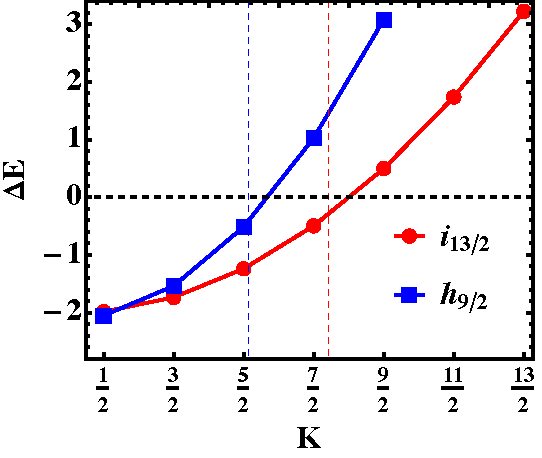
\includegraphics[scale=0.8]{Chapters/Figures/energy_shift_nilssonDeltaE.pdf} % figure was generated with the Mathematica script from here: /Users/basavyr/Documents/Work/mathematica-useful-algorithms/Physics/nilsson-energy-shift/energy-shift.nb
    \caption{The energy shift $\Delta E$ for two orbits: $h_{9/2}$ and $i_{13/2}$ for a given deformation $\epsilon=0.22$. The dashed vertical lines (colored) represent the value for $K$ where the `change' from downward sloping curves to upward sloping curves takes place (that is $K\approx 0.65j$). This is just an illustrative example inspired from the discussion regarding single-particle orbits in Ref. \cite{casten2000nuclear}}
    \label{fig-nilsson-delta-E-shift}
\end{figure}

Based on the principal quantum number $N$, there is another important physical consequence. The dependence on $N$ will imply that the slopes of any Nilsson energy level will be \emph{steeper} for larger values of $N$. Thus, heavier nuclei will tend to deform much easier than lighter ones. The explanation was done in Refs. \cite{bohr1998nuclear,krane1991introductory,casten2000nuclear}. Shortly, a nucleon belonging to a high oscillator shell will have a large average radius (the expectation value of $r^2$ was provided in Eq. \eqref{nilsson-energy-shifts} via the expression $\langle r^2 \rangle=(N+3/2)$ \cite{bertulani2007nuclear}). As the nucleus deforms, the density distribution of the nuclear matter will approach that orbit. The effect on the orbiting nucleon to decrease its energy rapidly as the nuclear matter comes closer to the orbit is due to the \emph{attractive} nature of the nuclear force. 
Clearly, this effect is less obvious for a particle in a lower oscillator shell that is already very close to the rest of the nuclear matter.

The centrifugal $\vec{l}^2$ and spin-orbit $\vec{l}\cdot\vec{s}$ terms from Eq. \eqref{eq-nilsson-ham-spherical-harmonics} will become negligible in the limit of \emph{large deformation}, such that the Nilsson Hamiltonian will become just like an AHO. In this special case, the motion will separate into \emph{independent} oscillations in the direction of the symmetry axis and the perpendicular plane (i.e., in the direction of $z$-axis and $xy$ plane). Consequently, the good quantum numbers for this kind of situation are the $n_z$ and $(n_x+n_y)$ oscillator quantum numbers. Since the eigenvalues for a one-dimensional (and, implicitly for the three-dimensional) harmonic oscillator are established, the energy spectrum for single-particle orbits in the regime of large $\epsilon$ will be given by \cite{casten2000nuclear}:
\begin{align}
    E_{n_x,n_y,n_z}=\hbar\omega_x(N-n_z+1)+\hbar\omega_z\left(n_z+\frac{1}{2}\right)\ .
\end{align}

The remarking feature of the Hamiltonian is its invariance to rotations about the $z$ axis. The projections for the particle's orbital and spin a.m. are constants of motion. As it was discussed, the sum of the two projections $\Lambda$ and $\Sigma$ is indeed $\Omega$ or, equivalently, $K$ in the case of $\vec{R}$ being perpendicular to the $z$-axis. Concluding, the importance of the Nilsson Deformed Model was made clear enough in this section. Its importance within the rest of the present work will be justified later on, where based on a Particle-Rotor-Model \cite{bohr1998nuclear,davydov1958rotational}, it will play a crucial role in determining the Hamiltonians specific to the nuclei of interest.
